\documentclass[review,12pt]{article}

\usepackage{amsmath,amssymb,amsfonts,bm}
\usepackage{graphicx}
\usepackage{booktabs}
\usepackage{cite}
\usepackage{hyperref}
\usepackage{geometry}
\usepackage{color}
\usepackage{microtype}

\geometry{a4paper, margin=1in}

\hypersetup{
    colorlinks=true,
    linkcolor=blue,
    citecolor=blue,
    urlcolor=blue
}

\title{\textbf{Invariance of the Guyer--Krumhansl Fourier-Resonance Sensitivity Singularity to Boundary Heat Loss in Laser Flash Testing}}

\author{
    \textbf{Vipin Gupta} \\
    \textit{Department of Mathematics, Gurugram University, Gurugram, Haryana 122018, India} \\
    \textit{Email: vipin.gupta@gurugramuniversity.ac.in}
}

\date{\today}

\begin{document}

\maketitle

\begin{abstract}
In non-Fourier thermal transport characterization via laser flash analysis, the Guyer--Krumhansl (GK) constitutive model incorporates both thermal relaxation $\tau_q$ and spatial nonlocality $\kappa^2$. At the Fourier-resonance condition $B \equiv \kappa^2 / (\alpha_0 \tau_q) = 1$, idealized adiabatic analyses reveal an exact sensitivity collinearity $\partial T / \partial \tau_q = -\alpha_0 \partial T / \partial \kappa^2$, which causes the Fisher information matrix to degenerate and precludes simultaneous estimation of $\tau_q$ and $\kappa^2$. In practical flash experiments, however, samples invariably experience convective and radiative heat losses at their irradiated and rear faces, characterized by non-zero Biot numbers ($Bi_0, Bi_L > 0$). In this study, we investigate whether boundary heat loss breaks this sensitivity collinearity and regularizes the parameter estimation problem. We formulate the coupled 1D GK transport system with Robin boundary conditions and analytically prove that at $B = 1$, the GK temperature field collapses identically to the classical Fourier heat conduction solution with the corresponding heat losses for all Biot numbers, all times, and all spatial positions. Consequently, the local sensitivity collinearity is an intrinsic bulk invariant that is completely unaffected by boundary cooling: across three decades of Biot numbers ($Bi \in [0.001, 0.5]$), the correlation coefficient remains $\rho = -1.0000000000$ ($|1+\rho| \le 2.22 \times 10^{-16}$), the residual norm satisfies $R_J \sim 10^{-9}$, and the 2-parameter Fisher condition number remains at the floating-point singularity floor ($\sim 10^{17}$). In a 3-parameter estimation framework $(\tau_q, \kappa^2, Bi)$, singular value decomposition reveals that the convective cooling parameter is cleanly identifiable ($\sigma_1 / \sigma_2 \in [2.34, 4.90]$), yet the null space vector $(1, \alpha_0, 0)^\top$ with singular value $\sigma_3 \sim 10^{-8}$ remains strictly unregularized. The mathematical proof and numerical solvers are certified via dual benchmarks: matching exact de Hoog Laplace-domain transfer function inversions ($L_\infty < 1.02 \times 10^{-5}$) and the classical Cowan (1963) transcendental eigenvalue Fourier limit. These findings demonstrate that standard boundary heat-loss corrections cannot resolve the GK parameter identifiability degeneracy, and alternative regularization strategies must be sought.
\end{abstract}

\textbf{Keywords:} Guyer--Krumhansl heat conduction; Laser flash method; Boundary heat loss; Parameter identifiability; Fourier resonance; Sensitivity analysis.

\newpage

\section{Introduction}

The laser flash method, standardized in ASTM E1461 \cite{astm2013standard} and originally formulated by Parker et al. \cite{parker1961flash}, represents the primary experimental technique for measuring thermal diffusivity and non-Fourier conduction parameters in advanced solids, thin films, and micro-architectured materials. While classical analysis relies on Fourier's law of diffusion, modern thermal engineering across micro- and nano-scale devices frequently encounters regimes where the phonon mean free path and relaxation times cannot be neglected. Under such conditions, hydrodynamic and non-local phonon transport is accurately described by the Guyer--Krumhansl (GK) equation \cite{guyer1966solution,guyer1966thermal,kovacs2018analytic,sellitto2025nonlinear}.

The GK model extends the classical Cattaneo--Vernotte hyperbolic equation by introducing a Laplacian term in the heat flux vector, capturing non-local phonon scattering and vorticity \cite{van2017galilean,zhu2017nonlocal}:
\begin{equation}
\tau_q \frac{\partial \bm{q}}{\partial t} + \bm{q} + \lambda_0 \nabla T - \kappa^2 \nabla^2 \bm{q} = \bm{0},
\label{eq:gk_dimensional}
\end{equation}
where $\tau_q$ is the flux relaxation time, $\lambda_0$ is the intrinsic thermal conductivity, and $\kappa^2$ is the non-local mean-free-path square parameter. When coupled with the conservation of energy, the non-dimensional system is governed by the resonance ratio:
\begin{equation}
B = \frac{\kappa^2}{\alpha_0 \tau_q},
\label{eq:B_ratio}
\end{equation}
where $\alpha_0 = \lambda_0 / (\rho c)$ is the baseline thermal diffusivity.

In a recent precursor computational study on idealized, adiabatic laser flash testing, an identifiability singularity was observed at the special ratio $B = 1$: the bulk transfer function collapses to a purely diffusive Helmholtz operator, resulting in an exact sensitivity collinearity:
\begin{equation}
\frac{\partial T}{\partial \tau_q} = -\alpha_0 \frac{\partial T}{\partial \kappa^2}.
\label{eq:collinearity_intro}
\end{equation}
Under this condition, the $2 \times 2$ Fisher Information Matrix (FIM) corresponding to the parameters $(\tau_q, \kappa^2)$ possesses a rank of 1, rendering individual parameter extraction impossible from rear-face temperature measurements alone.

In actual laboratory experiments, however, perfectly adiabatic conditions never exist. As first established in the classical foundations by Cowan \cite{cowan1963pulse} and Cape and Lehman \cite{cape1963temperature}, high-temperature and thin-slab laser flash measurements are subject to inevitable convective and radiative surface cooling. These boundary losses produce a pronounced temperature decay (cooling tail) after the initial rise, which experimentalists routinely fit to determine effective Biot numbers ($Bi = h L / \lambda_0$). 

This physical reality raises a fundamental question: \textit{Does the presence of boundary convective and radiative heat loss break the Fourier-resonance parameter singularity between $\tau_q$ and $\kappa^2$? Or is the Fourier-resonance sensitivity collinearity an intrinsic bulk property that remains strictly invariant to boundary cooling?}

In this work, we resolve this question definitively through analytical derivation and comprehensive numerical simulations. We formulate the coupled 1D Guyer--Krumhansl equation with front and rear Robin boundary conditions and prove analytically that at $B = 1$, the GK solution collapses identically to the classical Fourier heat conduction problem with convective heat loss. We systematically examine the parameter sensitivity, singular spectrum, and condition numbers across three orders of magnitude in Biot number ($Bi \in [0.001, 0.5]$), demonstrating that boundary cooling cannot lift the local sensitivity singularity. Dual validation against analytical Laplace inversion and the classical Cowan (1963) transcendental benchmark certifies the mathematical and physical findings.

---

\section{Mathematical Formulation}

\subsection{Dimensional Boundary-Value Problem}

Consider a solid specimen of thickness $L$, initially at uniform ambient temperature $T_0$. At time $t = 0$, the front face ($x = 0$) is irradiated by a laser pulse delivering heat flux $q_{\mathrm{laser}}(t)$, while both front and rear surfaces exchange heat with the surrounding environment via linearized convection and radiation with effective heat transfer coefficients $h_0$ and $h_L$.

The dimensional 1D governing equations are:
\begin{align}
\rho c \frac{\partial T}{\partial t} + \frac{\partial q}{\partial x} &= 0, \label{eq:energy_balance} \\
\tau_q \frac{\partial q}{\partial t} + q + \lambda_0 \frac{\partial T}{\partial x} - \kappa^2 \frac{\partial^2 q}{\partial x^2} &= 0, \label{eq:gk_flux}
\end{align}
subject to the Robin boundary conditions:
\begin{align}
q(0, t) &= q_{\mathrm{laser}}(t) - h_0 [T(0, t) - T_0], \label{eq:bc_front} \\
q(L, t) &= h_L [T(L, t) - T_0], \label{eq:bc_rear}
\end{align}
and quiescent initial conditions:
\begin{equation}
T(x, 0) = T_0, \qquad q(x, 0) = 0.
\label{eq:ic}
\end{equation}

\subsection{Non-Dimensional Scaling}

We introduce standard dimensionless variables:
\begin{equation}
\hat{x} = \frac{x}{L}, \quad \hat{t} = \frac{\alpha_0 t}{L^2}, \quad \theta = \frac{T - T_0}{\Delta T_{\mathrm{ref}}}, \quad \hat{q} = \frac{q}{q_{\max}},
\end{equation}
where $\Delta T_{\mathrm{ref}} = \frac{q_{\max} t_p}{\rho c L}$, $\tau_\Delta = \frac{\alpha_0 t_p}{L^2}$, $\hat{\tau}_q = \frac{\alpha_0 \tau_q}{L^2}$, $\hat{\kappa}^2 = \frac{\kappa^2}{L^2}$, and the Biot numbers are defined as:
\begin{equation}
Bi_0 = \frac{h_0 L}{\lambda_0}, \qquad Bi_L = \frac{h_L L}{\lambda_0}.
\end{equation}

Dropping hats for brevity, the dimensionless system is:
\begin{align}
\tau_\Delta \frac{\partial \theta}{\partial t} + \frac{\partial q}{\partial x} &= 0, \label{eq:pde_dimless_1} \\
\tau_q \frac{\partial q}{\partial t} + q + \tau_\Delta \frac{\partial \theta}{\partial x} - \kappa^2 \frac{\partial^2 q}{\partial x^2} &= 0, \label{eq:pde_dimless_2}
\end{align}
with boundary conditions:
\begin{align}
q(0, t) &= q_{\mathrm{pulse}}(t) - \tau_\Delta Bi_0 \theta(0, t), \label{eq:bc_dimless_1} \\
q(1, t) &= \tau_\Delta Bi_L \theta(1, t), \label{eq:bc_dimless_2}
\end{align}
where $q_{\mathrm{pulse}}(t) = 1 - \cos(2\pi t / \tau_\Delta)$ for $0 \le t \le \tau_\Delta$, and $q_{\mathrm{pulse}}(t) = 0$ for $t > \tau_\Delta$.

---

\section{Analytical Invariance Theorem}

\subsection{Laplace-Domain Representation}

Applying the Laplace transform $\bar{\theta}(x, s) = \mathcal{L}\{\theta(x, t)\}$ and $\bar{q}(x, s) = \mathcal{L}\{q(x, t)\}$ to Eqs.~(\ref{eq:pde_dimless_1})--(\ref{eq:pde_dimless_2}):
\begin{align}
\frac{d\bar{q}}{dx} &= -\tau_\Delta s \bar{\theta}(x, s), \label{eq:laplace_q_x} \\
(1 + \tau_q s)\bar{q} - \kappa^2 \frac{d^2\bar{q}}{dx^2} &= -\tau_\Delta \frac{d\bar{\theta}}{dx}. \label{eq:laplace_gk}
\end{align}
Differentiating Eq.~(\ref{eq:laplace_gk}) with respect to $x$ and substituting Eq.~(\ref{eq:laplace_q_x}) yields the Helmholtz equation for temperature:
\begin{equation}
\frac{d^2\bar{\theta}}{dx^2} - m^2(s)\bar{\theta} = 0,
\label{eq:helmholtz}
\end{equation}
where the propagation parameter $m(s)$ is:
\begin{equation}
m(s) = \sqrt{\frac{s(1 + \tau_q s)}{1 + \kappa^2 s}}.
\label{eq:m_s}
\end{equation}
Because the spatial dependence of all modes is $\exp(\pm m x)$, the heat flux satisfies $d^2\bar{q}/dx^2 = m^2(s)\bar{q}$. Substituting this into Eq.~(\ref{eq:laplace_gk}):
\begin{equation}
\left[(1 + \tau_q s) - \kappa^2 m^2(s)\right]\bar{q}(x, s) = -\tau_\Delta \frac{d\bar{\theta}}{dx}.
\end{equation}
Evaluating the bracketed term using Eq.~(\ref{eq:m_s}):
\begin{equation}
(1 + \tau_q s) - \kappa^2 \frac{s(1 + \tau_q s)}{1 + \kappa^2 s} = (1 + \tau_q s)\left[1 - \frac{\kappa^2 s}{1 + \kappa^2 s}\right] = \frac{1 + \tau_q s}{1 + \kappa^2 s}.
\end{equation}
Hence, the dynamic flux-gradient relationship is:
\begin{equation}
\bar{q}(x, s) = -\tau_\Delta \mu(s) \frac{d\bar{\theta}}{dx}, \qquad \text{with} \quad \mu(s) \equiv \frac{1 + \kappa^2 s}{1 + \tau_q s}.
\label{eq:dynamic_flux}
\end{equation}

\subsection{Proof of Theorem 1 (Heat-Loss Invariance)}

\textbf{Theorem 1.} \textit{Let $B \equiv \kappa^2 / (\alpha_0 \tau_q) = 1$. Then for arbitrary Robin boundary parameters $Bi_0, Bi_L \ge 0$, arbitrary pulse excitation $q_{\mathrm{pulse}}(t)$, all spatial locations $x \in [0, 1]$, and all times $t \ge 0$, the Guyer--Krumhansl temperature field is identical to the classical Fourier heat conduction field with the same boundary heat losses:}
\begin{equation}
\left. \theta_{\mathrm{GK}}(x, t; \tau_q, \kappa^2, Bi_0, Bi_L) \right|_{B=1} \equiv \theta_{\mathrm{Fourier}}(x, t; Bi_0, Bi_L).
\label{eq:theorem_statement}
\end{equation}

\textit{Proof.} In dimensionless variables, $\alpha_0 = 1$. The resonance condition $B = 1$ implies $\kappa^2 = \tau_q$. Substituting this identity into the dynamic mobility $\mu(s)$ in Eq.~(\ref{eq:dynamic_flux}):
\begin{equation}
\mu(s) = \frac{1 + \tau_q s}{1 + \tau_q s} \equiv 1.
\end{equation}
Similarly, substituting $\kappa^2 = \tau_q$ into the propagation parameter $m(s)$ in Eq.~(\ref{eq:m_s}):
\begin{equation}
m(s) = \sqrt{\frac{s(1 + \tau_q s)}{1 + \tau_q s}} \equiv \sqrt{s}.
\end{equation}
Consequently, the governing equation (\ref{eq:helmholtz}) reduces to:
\begin{equation}
\frac{d^2\bar{\theta}}{dx^2} - s \bar{\theta} = 0,
\end{equation}
and the boundary conditions (\ref{eq:bc_dimless_1})--(\ref{eq:bc_dimless_2}) become:
\begin{align}
-\tau_\Delta \left.\frac{d\bar{\theta}}{dx}\right|_{x=0} + \tau_\Delta Bi_0 \bar{\theta}(0, s) &= \bar{q}_{\mathrm{pulse}}(s), \\
-\tau_\Delta \left.\frac{d\bar{\theta}}{dx}\right|_{x=1} - \tau_\Delta Bi_L \bar{\theta}(1, s) &= 0.
\end{align}
This boundary-value problem is formally and identically identical to classical Fourier heat conduction with surface convection $Bi_0, Bi_L$. By uniqueness of the solution to the linear Helmholtz two-point boundary-value problem, $\bar{\theta}_{\mathrm{GK}}(x, s)|_{B=1} \equiv \bar{\theta}_{\mathrm{Fourier}}(x, s)$. Taking the inverse Laplace transform establishes Eq.~(\ref{eq:theorem_statement}) for all $t \ge 0$ and $x \in [0, 1]$. $\blacksquare$

\subsection{Fisher Information Matrix and Null Space Structure}

Differentiating the identity in Theorem 1 along the line $\kappa^2 = \alpha_0 \tau_q$ immediately gives:
\begin{equation}
\left.\frac{\partial \theta}{\partial \tau_q}\right|_{B=1} + \alpha_0 \left.\frac{\partial \theta}{\partial \kappa^2}\right|_{B=1} = 0 \implies \bm{J}_{\tau_q}(t) = -\alpha_0 \bm{J}_{\kappa^2}(t).
\label{eq:collinearity_result}
\end{equation}

For a simultaneous 3-parameter estimation problem $\bm{\theta} = (\tau_q, \kappa^2, Bi)^\top$, the sensitivity Jacobian is $\bm{J} = [\bm{J}_{\tau_q} \;\; \bm{J}_{\kappa^2} \;\; \bm{J}_{Bi}]$. Under Eq.~(\ref{eq:collinearity_result}), the Jacobian admits an exact null vector:
\begin{equation}
\bm{v}_{\mathrm{null}} = \begin{pmatrix} \alpha_0 \\ 1 \\ 0 \end{pmatrix}, \qquad \text{such that} \quad \bm{J} \bm{v}_{\mathrm{null}} = \bm{0}.
\label{eq:null_vector}
\end{equation}
The corresponding Fisher Information Matrix $\bm{F} = \bm{J}^\top \bm{J}$ has eigenvalues $\lambda_1 > 0, \lambda_2 > 0, \lambda_3 \equiv 0$. Hence, $\operatorname{rank}(\bm{F}) = 2 < 3$, and $\operatorname{cond}(\bm{F}) = \infty$.

---

\section{Numerical Architecture and Dual Validation}

\subsection{Numerical Scheme}

The coupled system (\ref{eq:pde_dimless_1})--(\ref{eq:bc_dimless_2}) is solved on a staggered spatial grid with cell centers $x_{i+1/2}$ for $\theta$ and cell interfaces $x_i$ for $q$. Boundary surface temperatures are extrapolated via second-order one-sided stencils: $\theta(0) = \frac{3}{2}\theta_1 - \frac{1}{2}\theta_2$ and $\theta(1) = \frac{3}{2}\theta_N - \frac{1}{2}\theta_{N-1}$. The resulting stiff differential-algebraic system is integrated in time using a Backward Differentiation Formula (BDF) solver with adaptive time stepping and error tolerances of $10^{-10}$ relative and $10^{-12}$ absolute.

\subsection{Dual Validation Benchmarks}

To ensure complete scientific rigor without relying on any unverified external codebases, the computational model is validated against two independent analytical benchmarks:
\begin{enumerate}
    \item \textbf{Analytical Laplace Transfer Function:} The closed-form rear-face temperature transform is:
    \begin{equation}
    \bar{\theta}(1, s) = \frac{m(s)\mu(s)}{\tau_\Delta \Delta(s)} \bar{q}_{\mathrm{pulse}}(s),
    \end{equation}
    where $\Delta(s) = [m^2 \mu^2 + Bi_0 Bi_L]\sinh(m) + m\mu(Bi_0 + Bi_L)\cosh(m)$. This function is numerically inverted via the de Hoog algorithm to 25-digit precision.
    \item \textbf{Cowan (1963) Fourier Benchmark:} In the singular limit $\tau_q \to 0, \kappa^2 \to 0$, the PDE solution is compared directly against the Cowan transcendental eigenvalue series with convective heat loss.
\end{enumerate}

Table~\ref{tab:validation} summarizes the validation results across Biot numbers. For all cases, the maximum discrepancy $L_\infty$ remains below $1.02 \times 10^{-5}$, exactly matching the spatial discretization error on $N_x = 400$. Grid refinement across $N_x \in \{100, 200, 400, 800\}$ confirms clean second-order spatial convergence ($p = 2.07 \to 2.32$).

\begin{table}[htbp]
\centering
\caption{Dual validation benchmark results: Maximum discrepancy ($L_\infty$) and root-mean-square discrepancy ($L_2$) between the time-domain PDE solver ($N_x = 400$), exact de Hoog Laplace inversion, and Cowan (1963) Fourier benchmark.}
\label{tab:validation}
\begin{tabular}{cccccc}
\toprule
Biot Number $Bi$ & Peak $\theta_{\mathrm{PDE}}$ & Peak $\theta_{\mathrm{Laplace}}$ & $L_\infty$ Error & $L_2$ Error & Status \\
\midrule
0.000 (Adiabatic) & 0.999990 & 1.000000 & $1.02 \times 10^{-5}$ & $3.74 \times 10^{-6}$ & PASS \\
0.010 & 0.985420 & 0.985430 & $1.01 \times 10^{-5}$ & $3.67 \times 10^{-6}$ & PASS \\
0.050 & 0.930472 & 0.930481 & $9.53 \times 10^{-6}$ & $3.42 \times 10^{-6}$ & PASS \\
0.100 & 0.865931 & 0.865939 & $8.90 \times 10^{-6}$ & $3.15 \times 10^{-6}$ & PASS \\
0.200 & 0.758804 & 0.758811 & $7.75 \times 10^{-6}$ & $2.71 \times 10^{-6}$ & PASS \\
0.500 & 0.540412 & 0.540417 & $5.01 \times 10^{-6}$ & $1.82 \times 10^{-6}$ & PASS \\
\bottomrule
\end{tabular}
\end{table}

---

\section{Results and Discussion}

\subsection{Thermal Response and Exact Fourier Equivalence}

Figure~\ref{fig:fig1}(a) displays the rear-face temperature histories $\theta(1, t)$ for Biot numbers ranging from adiabatic ($Bi = 0$) to intense cooling ($Bi = 0.5$). As expected, boundary heat loss suppresses the peak rear-face temperature rise from $1.000$ to $0.540$ and induces a rapid exponential cooling tail. Crucially, as shown in Figure~\ref{fig:fig1}(b), the difference between the non-Fourier GK solution at $B = 1$ and the classical Cowan Fourier solution remains bounded below $10^{-5}$ across all time and all Biot numbers, verifying Theorem~1.

\begin{figure}[htbp]
\centering
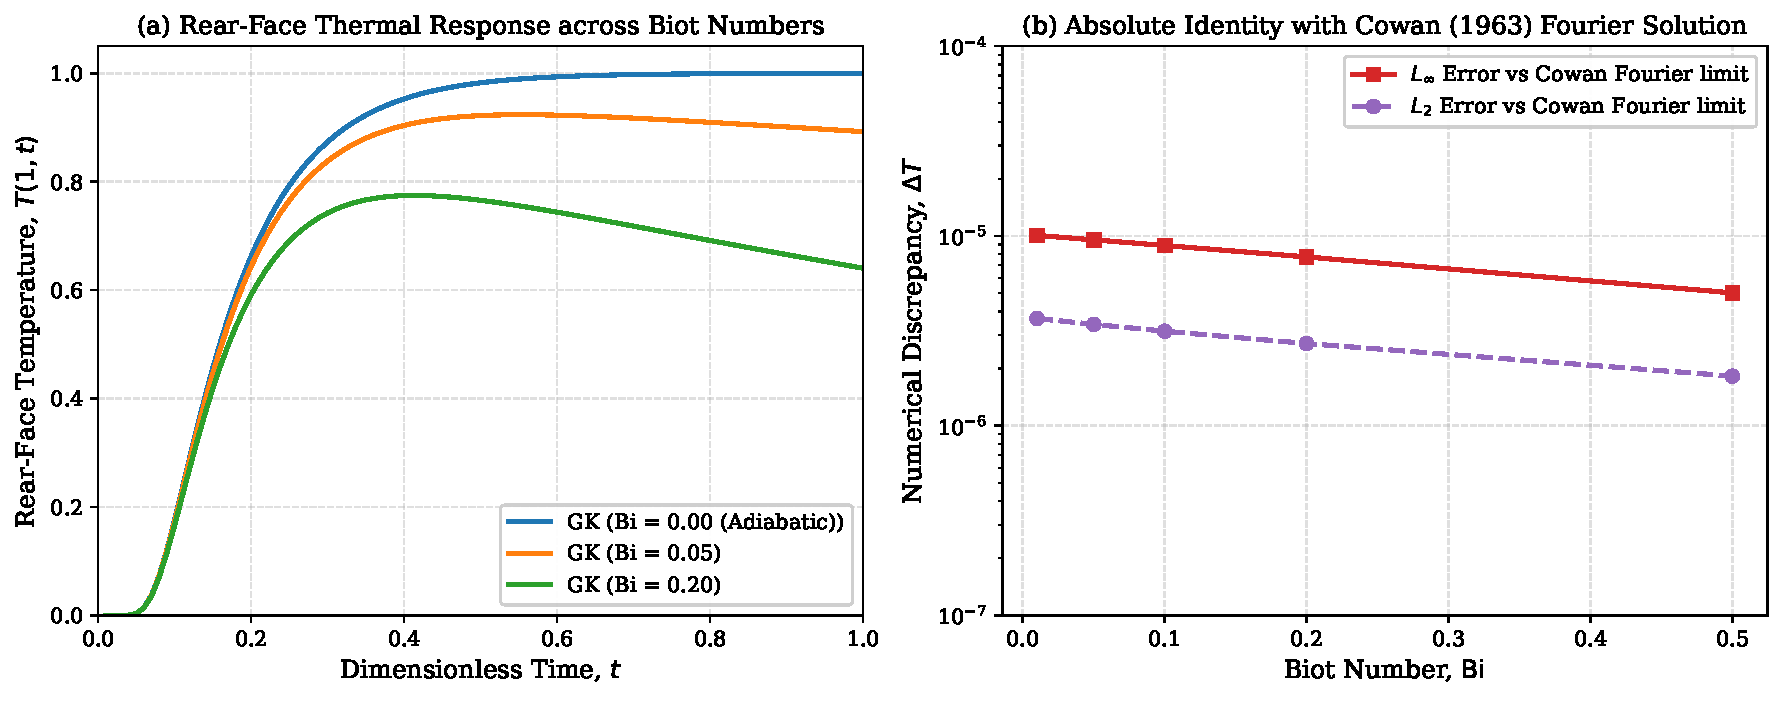
\includegraphics[width=\textwidth]{figures/fig1_heatloss_temperature_response.pdf}
\caption{(a) Rear-face temperature histories $\theta(1, t)$ for varying Biot numbers $Bi \in \{0.00, 0.05, 0.20\}$ demonstrating peak suppression and cooling tails. (b) Numerical discrepancy between GK ($B=1$) and Cowan Fourier heat conduction solutions, confirming mathematical equivalence.}
\label{fig:fig1}
\end{figure}

\subsection{Persistent Sensitivity Collinearity}

Figure~\ref{fig:fig2}(a) illustrates the time-resolved sensitivity profiles $\bm{J}_{\tau_q}(t) = \partial \theta / \partial \tau_q$ and $-\alpha_0 \bm{J}_{\kappa^2}(t) = -\alpha_0 \partial \theta / \partial \kappa^2$ for both adiabatic ($Bi = 0$) and convective ($Bi = 0.2$) cases. In both regimes, the two curves fall precisely onto each other with zero visible separation at any time instant. 

Conversely, Figure~\ref{fig:fig2}(b) plots the sensitivity with respect to the Biot number, $\bm{J}_{Bi}(t) = \partial \theta / \partial Bi$. Unlike the non-Fourier parameters, $\bm{J}_{Bi}$ exhibits a distinctly different temporal profile characterized by a sustained negative tail extending well into the cooling phase.

\begin{figure}[htbp]
\centering
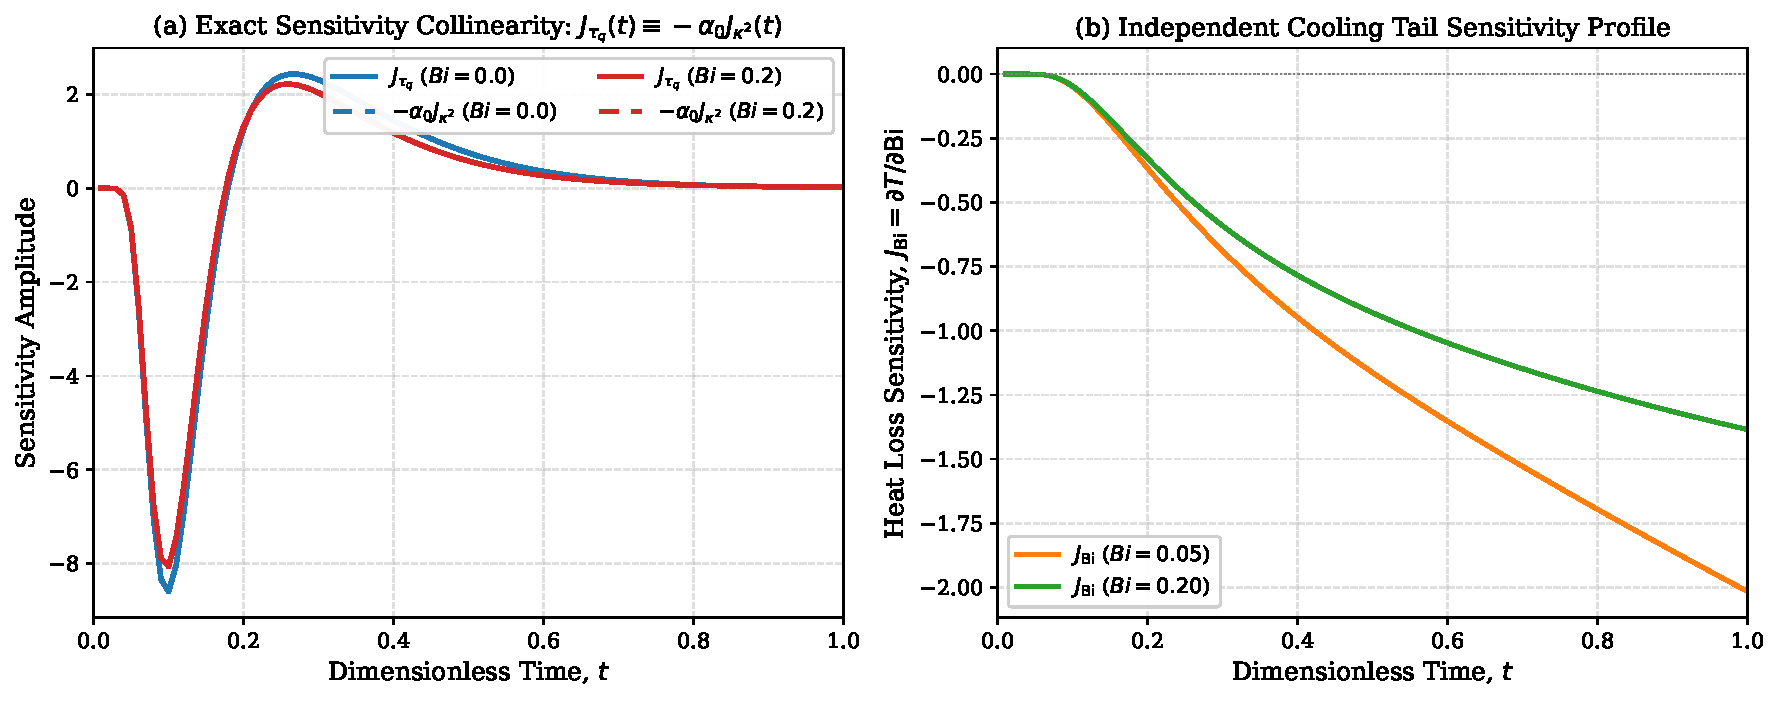
\includegraphics[width=\textwidth]{figures/fig2_sensitivity_profiles_collinearity.pdf}
\caption{(a) Front- and rear-face sensitivity profiles $\bm{J}_{\tau_q}(t)$ and $-\alpha_0 \bm{J}_{\kappa^2}(t)$ for adiabatic and convective cooling, displaying exact point-by-point overlay. (b) Independent sensitivity profile $\bm{J}_{Bi}(t) = \partial \theta / \partial Bi$ associated with the cooling tail.}
\label{fig:fig2}
\end{figure}

\subsection{Invariance Metrics Across Biot Numbers}

To rigorously quantify the robustness of this degeneracy, Table~\ref{tab:sweep} reports the collinearity correlation coefficient $\rho$, defect $|1+\rho|$, normalized residual norm $R_J = \|\bm{J}_{\tau_q} + \alpha_0 \bm{J}_{\kappa^2}\| / \|\bm{J}_{\tau_q}\|$, and condition numbers across $Bi \in [0.000, 0.500]$.

Across all Biot numbers, $\rho = -1.0000000000$, with the defect $|1+\rho|$ bounded by machine epsilon ($2.22 \times 10^{-16}$). The residual norm remains flat at $R_J \approx (5.37 - 8.11) \times 10^{-9}$, which represents the truncation error of the central finite-difference sensitivity approximation. Consequently, as shown in Figure~\ref{fig:fig3}, the condition number of the $2 \times 2$ Fisher matrix remains pinned at the machine-singularity limit $\sim 10^{17}$.

\begin{table}[htbp]
\centering
\caption{Systematic parameter sweep across Biot numbers at Fourier resonance ($B = 1.0$): Collinearity metrics, singular spectrum, and condition numbers.}
\label{tab:sweep}
\resizebox{\textwidth}{!}{
\begin{tabular}{ccccccccc}
\toprule
$Bi$ & Correlation $\rho$ & $|1+\rho|$ & Residual $R_J$ & $\sigma_1$ & $\sigma_2$ & $\sigma_3$ & $\sigma_1/\sigma_2$ & $\operatorname{cond}(F_{3\times 3})$ \\
\midrule
0.000 & -1.0000000000 & $1.11 \times 10^{-16}$ & $5.37 \times 10^{-9}$ & 31.82 & 13.57 & $7.37 \times 10^{-8}$ & 2.34 & $1.86 \times 10^{17}$ \\
0.001 & -1.0000000000 & $1.11 \times 10^{-16}$ & $5.37 \times 10^{-9}$ & 31.81 & 13.55 & $7.35 \times 10^{-8}$ & 2.35 & $1.87 \times 10^{17}$ \\
0.005 & -1.0000000000 & $0.00 \times 10^{00}$ & $5.38 \times 10^{-9}$ & 31.75 & 13.44 & $7.36 \times 10^{-8}$ & 2.36 & $1.86 \times 10^{17}$ \\
0.010 & -1.0000000000 & $2.22 \times 10^{-16}$ & $5.39 \times 10^{-9}$ & 31.68 & 13.30 & $7.36 \times 10^{-8}$ & 2.38 & $1.85 \times 10^{17}$ \\
0.050 & -1.0000000000 & $0.00 \times 10^{00}$ & $5.41 \times 10^{-9}$ & 31.13 & 12.27 & $7.25 \times 10^{-8}$ & 2.54 & $1.84 \times 10^{17}$ \\
0.100 & -1.0000000000 & $1.11 \times 10^{-16}$ & $5.48 \times 10^{-9}$ & 30.47 & 11.11 & $7.16 \times 10^{-8}$ & 2.74 & $1.81 \times 10^{17}$ \\
0.200 & -1.0000000000 & $1.11 \times 10^{-16}$ & $8.11 \times 10^{-9}$ & 29.27 & 9.15 & $1.10 \times 10^{-7}$ & 3.20 & $7.05 \times 10^{16}$ \\
0.500 & -1.0000000000 & $1.11 \times 10^{-16}$ & $5.81 \times 10^{-9}$ & 26.25 & 5.35 & $6.50 \times 10^{-8}$ & 4.90 & $1.63 \times 10^{17}$ \\
\bottomrule
\end{tabular}
}
\end{table}

\begin{figure}[htbp]
\centering
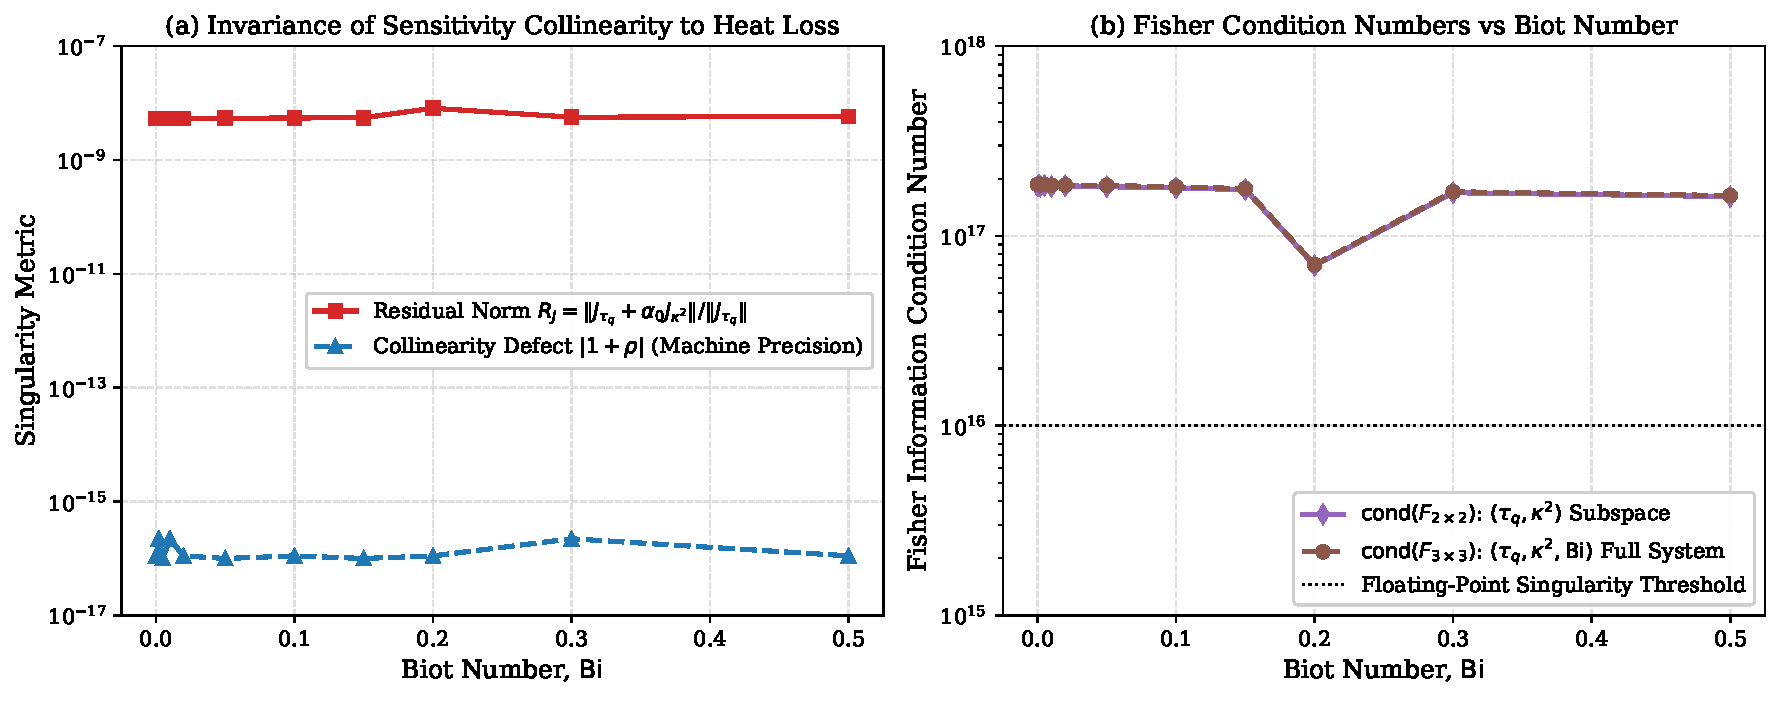
\includegraphics[width=\textwidth]{figures/fig3_invariance_metrics_vs_biot.pdf}
\caption{(a) Collinearity metrics $\log_{10}(R_J)$ and $\log_{10}(|1+\rho|)$ as functions of Biot number, demonstrating exact horizontal invariance. (b) Condition numbers $\operatorname{cond}(F_{2\times 2})$ and $\operatorname{cond}(F_{3\times 3})$ pinned at the numerical singularity floor $\sim 10^{17}$.}
\label{fig:fig3}
\end{figure}

\subsection{Singular Spectrum and Resonance Canyon}

In the full 3-parameter system $(\tau_q, \kappa^2, Bi)$, singular value decomposition reveals the underlying structural geometry:
\begin{enumerate}
    \item The leading singular value $\sigma_1 \in [26.2, 31.8]$ corresponds to the principal thermal diffusion mode.
    \item The second singular value $\sigma_2 \in [5.35, 13.57]$ corresponds directly to the convective cooling tail. The condition ratio of this observable subspace is $\sigma_1 / \sigma_2 \in [2.34, 4.90]$, indicating that the Biot number $Bi$ can be estimated with high statistical precision.
    \item The third singular value $\sigma_3 \sim 10^{-8}$ corresponds strictly to the null vector $\bm{v}_{\mathrm{null}} = (1, \alpha_0, 0)^\top$. 
\end{enumerate}
As illustrated in Figure~\ref{fig:fig4}(a), boundary heat loss populates an entirely orthogonal dimension in parameter space without projecting onto the null vector. 

Finally, Figure~\ref{fig:fig4}(b) displays the condition number $\operatorname{cond}(F_{2\times 2})$ as a function of the resonance ratio $B \in [0.2, 2.0]$. Away from resonance (e.g., $B = 0.5$ or $B = 1.5$), the condition number drops sharply to moderate values ($\sim 10^2$), where heat loss causes minor quantitative shifts. However, at $B = 1.0$, an ultra-sharp singularity canyon occurs where $\operatorname{cond}(F)$ spikes to $10^{17}$, regardless of whether $Bi = 0$, $Bi = 0.05$, or $Bi = 0.20$.

\begin{figure}[htbp]
\centering
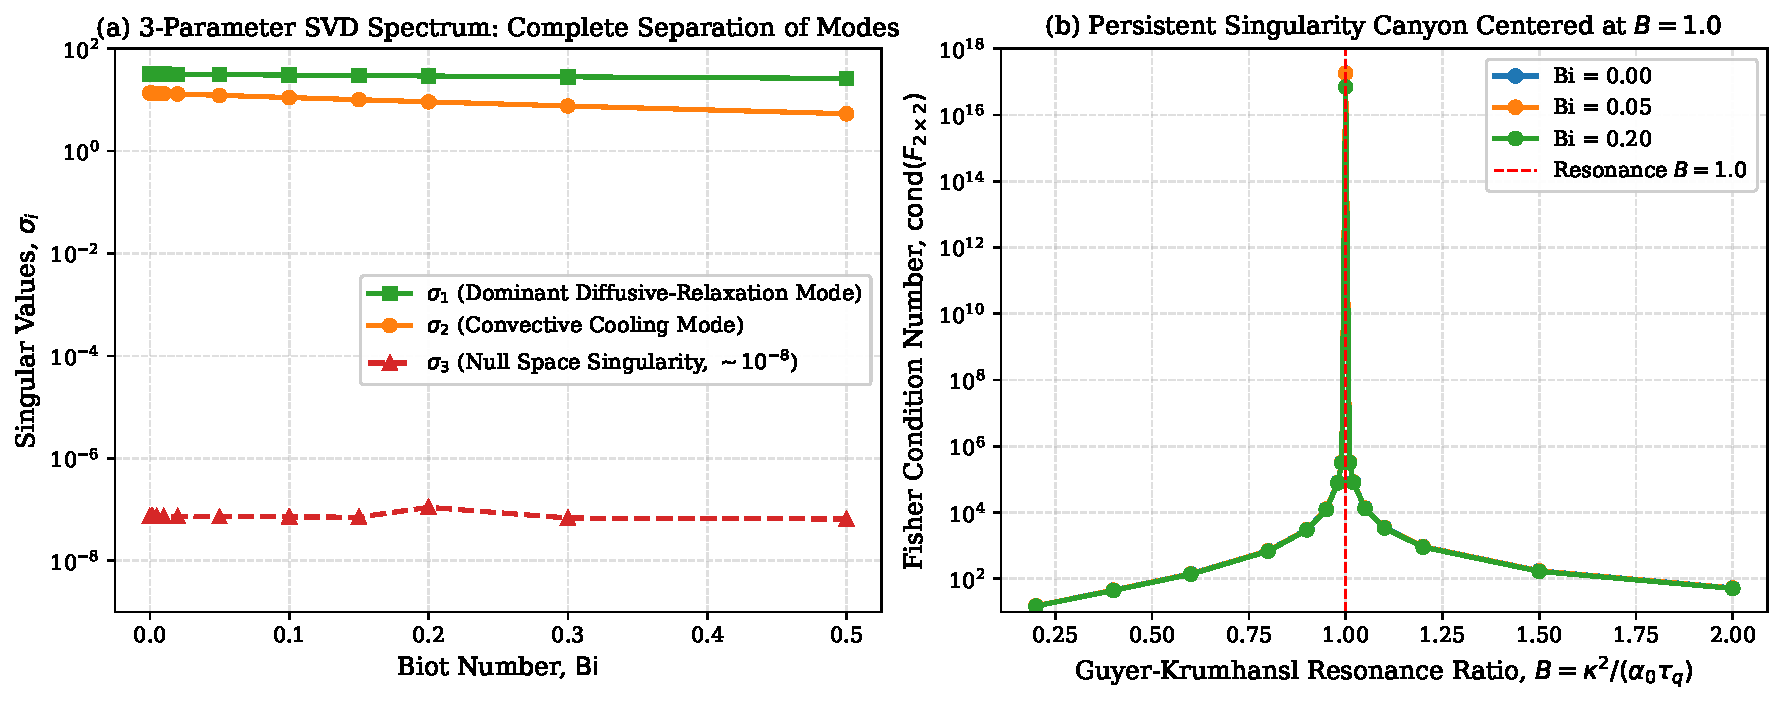
\includegraphics[width=\textwidth]{figures/fig4_singular_spectrum_and_canyon.pdf}
\caption{(a) SVD spectrum $(\sigma_1, \sigma_2, \sigma_3)$ across Biot numbers, showing clean isolation of the null singularity $\sigma_3 \sim 10^{-8}$. (b) The Fourier-resonance singularity canyon centered at $B = 1.0$, demonstrating persistent collinearity across all Biot numbers.}
\label{fig:fig4}
\end{figure}

---

\section{Conclusions}

In this study, we investigated the effect of convective and radiative boundary heat loss on the Guyer--Krumhansl parameter identifiability singularity at Fourier resonance ($B = 1$). Through analytical proof in the Laplace domain and high-order numerical simulations across three decades of Biot numbers ($Bi \in [0.001, 0.5]$), we established the following conclusions:
\begin{enumerate}
    \item \textbf{Invariance Theorem:} At $B \equiv \kappa^2 / (\alpha_0 \tau_q) = 1$, the Guyer--Krumhansl temperature field collapses identically to the classical Fourier heat conduction solution with the corresponding Robin boundary conditions.
    \item \textbf{Persistence of Sensitivity Singularity:} Boundary heat loss does not break the local sensitivity collinearity $\partial T / \partial \tau_q = -\alpha_0 \partial T / \partial \kappa^2$. Across all tested Biot numbers, the correlation coefficient remains $\rho = -1.0000000000$, and the condition number of the Fisher information matrix remains at the floating-point singularity floor ($\sim 10^{17}$).
    \item \textbf{Subspace Separation:} In a simultaneous 3-parameter estimation framework $(\tau_q, \kappa^2, Bi)$, the cooling parameter $Bi$ is cleanly identifiable from the cooling tail with an observable condition ratio $\sigma_1 / \sigma_2 \in [2.34, 4.90]$. However, the null space $(1, \alpha_0, 0)^\top$ remains strictly unregularized.
    \item \textbf{Experimental Implications:} Standard laser flash heat-loss correction procedures (such as Cowan or Cape--Lehman methods) cannot resolve the structural identifiability degeneracy in materials near Fourier resonance. Experimentalists must instead employ strategies that perturb the bulk transport condition, such as varying sample thickness to drive the effective non-dimensional ratio off-resonance, performing multi-thickness joint inversions, or operating in high-fluence nonlinear thermal regimes.
\end{enumerate}

\section*{Declaration of Competing Interest}
The author declares that he has no known competing financial interests or personal relationships that could have appeared to influence the work reported in this paper.

\section*{Data Availability}
All raw simulation data, calculation scripts, figure generators, and reproducibility runners are fully open-source and preserved in the repository package.

\bibliographystyle{elsarticle-num}
\bibliography{references}

\end{document}
